%%%%%%%%%%%%%%%%%%%%%%%%%%%%%%%%%%%%%%%%%%%%%%%%%%%%%%%
% A template for Wiley article submissions.
% Developed by Overleaf. 
%
% Please note that whilst this template provides a 
% preview of the typeset manuscript for submission, it 
% will not necessarily be the final publication layout.
%
% Usage notes:
% The "blind" option will make anonymous all author, affiliation, correspondence and funding information.
% Use "num-refs" option for numerical citation and references style.
% Use "alpha-refs" option for author-year citation and references style.

\documentclass[alpha-refs]{wiley-article}
% \documentclass[blind,num-refs]{wiley-article}

% Add additional packages here if required
\usepackage{siunitx}
\usepackage{lineno}

% Update article type if known
\papertype{Original Article}
% Include section in journal if known, otherwise delete
\paperfield{Pest Management Science}

\title{Spinosad baited spheres to attract and kill onion maggot \textit{Delia antiqua}}

% List abbreviations here, if any. Please note that it is preferred that abbreviations be defined at the first instance they appear in the text, rather than creating an abbreviations list.
%\abbrevs{ABC, a black cat; DEF, doesn't ever fret; GHI, goes home immediately.}

% Include full author names and degrees, when required by the journal.
% Use the \authfn to add symbols for additional footnotes and present addresses, if any. Usually start with 1 for notes about author contributions; then continuing with 2 etc if any author has a different present address.
\author[1\authfn{1}]{Denis S. Willett}
\author[1\authfn{1}]{Camila C. Filgueiras}
\author[2]{Starker Wright}
\author[1]{Jan P. Nyrop}
\author[1]{Brian A. Nault}

\contrib[\authfn{1}]{Equally contributing authors.}

% Include full affiliation details for all authors
\affil[1]{Department of Entomology, Cornell AgriTech, Cornell University, Geneva, NY, 14456, USA}
\affil[2]{Bartlett Tree Experts, Dublin, PA, USA}

\corraddress{Denis S. Willett, 15 Castle Creek Drive, Geneva, NY 14456}
\corremail{deniswillett@cornell.edu}


% Include the name of the author that should appear in the running header
\runningauthor{Willett et al.}

\begin{document}

\maketitle

\begin{abstract}

% Please include a maximum of seven keywords
\keywords{Onion Maggot, \textit{Delia antiqua}, attraction, sticky-trap, attract-and-kill, lure, onion management}
\end{abstract}

\linenumbers
\section{Introduction}
\section{Materials and Methods}

\subsection{Field Trials}

\paragraph{Shape Trial} To evaluate effect of trap shape on trap catch and monitoring of adult onion maggot fly, square, cube, short cylindrical, tall cylindrical, and spherical semi-gloss white shapes each with a surface area of 180 $cm^2$  were coated with sticky material (\textbf{Tanglefoot?}) and placed along the long edge of an onion (\textit{Allium cepa} L.) field near Elba, NY.  Traps were spaced 15.24 meters apart and arranged in a randomized control block design with five replications.  Traps were placed in the field in late May then collected in late June.   

\paragraph{Size Trial}
To evaluate the influence of trap size on the trap catch and monitoring of adult onion maggot fly, white spherical sticky traps with diameters of 5.00, 6.25, 7.50, 8.75, and 10.00 cm diameter were placed along the long edge of onion fields with spacing 15.24 meters apart in a randomized controlled block design with five replications.  

\paragraph{Color Trial}
To evaluate the effect of color on trap catch and monitoring of adult onion maggot fly, white, yellow, green, and red spherical sticky traps 8.75 cm in diameter were placed along the long edge of onion fields in a randomized controlled block design with five replications.  

\paragraph{Delia Lure Trial}
To evaluate the effect of adding an attractant an trap catch and monitoring of adult onion maggot flies, white spherical sticky traps 8.75 cm in diameter were placed at the edge of onion fields in a paired design where half of the traps received a Delia Lure (Baited) and the other half did not (Unbaited).  Trap Catch was monitored three times throughout the season and four replications of each treatment were conducted in each location.  


\subsection{Analysis}
\subsection{Data Management}


\section{Results}

\paragraph{Population Monitoring}

\paragraph{Onion Maggot Mortality}

\paragraph{Field Damage}



\begin{figure}[bt]
\centering
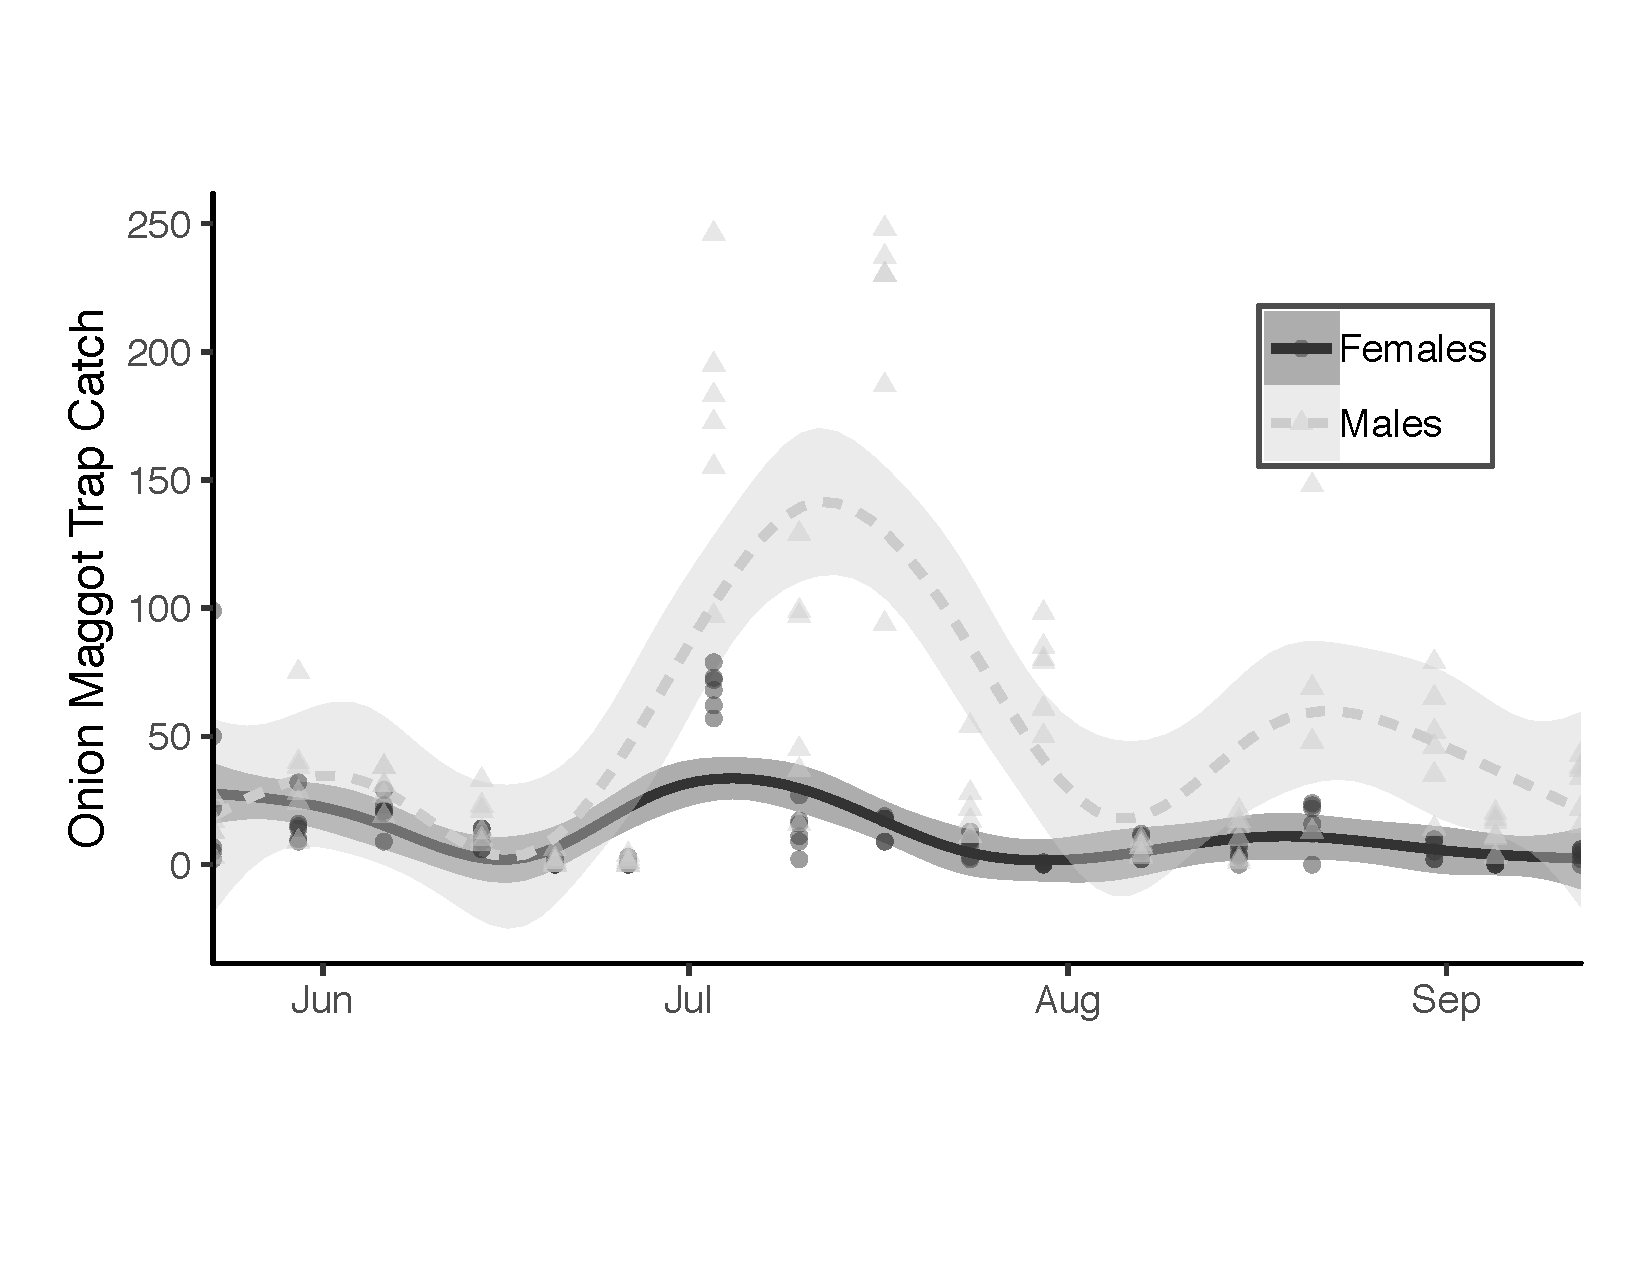
\includegraphics[width = 8cm]{figures/final-figures/figure-1.pdf}
\caption{ }
\label{fig:figure1}
\end{figure}

\paragraph{Shape Trial} Models relating trap shape and \textit{D. antiqua} sex to trap catch significantly explained approximately 70\% of observed variation (P \textless 0.001, $R^2_{adj}$ = 0.70, Table \ref{table:1}).  Trap shape significantly influenced (P = 0.005) catch of adult \textit{D. antiqua} (Figure \ref{fig:figure1}).  Sticky traps caught approximately 27.81 $\pm$ 2.8 more female flies than male flies.  Short cylindrical traps outperformed square panel and tall cylinder traps in terms of female trap catch.  While there were no significant differences between females captured on short cylinder, sphere, and cube traps, short cylinders tended to outperform cubes and spheres.  No significant differences were observed between male trap catch.  


\paragraph{Size Trial} Models using size, sex, and year to explain observed trap catch significantly explained approximately 73\% of the observed variation (P \textless 0.001, $R^2_{adj}$ = 0.73, Table \ref{table:1}).  Trap size significantly influenced trap catch (P \textless 0.001).  Increasing diameter of trap size showed a trend towards increasing trap catch (Figure \ref{fig:figure2}) with the largest trap catching significantly more females and males.  While male trap catch was less than that of females, trends in catch amoung the different diameters were similar for both males and females.  


\paragraph{Color Trial} Models using color and sex to explain observed trap catch significantly explained approximately 79\% of the observed variation (P \textless 0.001, $R^2_{adj}$ = 0.79, Table \ref{table:1}). Color significantly influenced trap catch (P \textless 0.001) with white traps catching significantly more females than any other color (t \textless -3.1, df = 32, P \textless 0.012) and significantly more males than any other color except yellow (t \textless -3.1, df = 32, P \textless 0.012, Yellow: t = -1.6, df = 32, P = 0.3).  White traps caught significantly more females than males (t = 6.1, df = 32, P \textless 0.001).

\paragraph{Delia Lure Trial} The presence of Delia Lure in conjunction with sticky traps increased catch of adult onion maggot flies.  Traps baited with Delia Lure caught approximately 51.3 (95\% CI: 7.3-95.4) more adult flies than traps without the Delia Lure bait (t = 3.0, df = 5, P = 0.03).


\section{Discussion}


\section*{Acknowledgements}
Suggestions for acknowledgements?

\section*{Conflict of Interest}
The authors declare no conflict of interest.  

\section*{Author Contribution}
BAN, JPN, and SW designed the experiments.  DSW, CCF, and BAN analyzed the data and wrote the manuscript.  


\section*{Data Availability Statement}
All code and data, including manuscript documentation, is available on GitHub(https://github.com/acetworld/onion-maggot-attraction).

%\printendnotes


\section{References}

\bibliographystyle{vancouver-authoryear}
\bibliography{om-attraction}

\graphicalabstract{example-image-1x1}{Please check the journal's author guildines for whether a graphical abstract, key points, new findings, or other items are required for display in the Table of Contents.}

\end{document}
